%----------------------------------------------------------------------------------------
%	CHAPTER
%----------------------------------------------------------------------------------------

\chapterimage{chapter_head_2.pdf} % Chapter heading image

\chapter{RAT: Robox Agv Tool}

\section{RAT}
RAT is a CAD software, fig.\ref{fig:refRat}, aimed to design maps and convert them into a formatted ASCII file with \textit{.map} extension. RAT save the created files as \textit{xml file}. A map can also be created using a text editor following some rules.\\

RAT can load \textit{dxf} files as background, that can be used as a guide to design the desired map. Mainly RAT have lines, points, vehicles. These component will be explained later.\\
		
In the properties of the project some settings have to be changed in order to change the behavior of the AGV motion, for example \textit{Trasversal navigation} is set by default to \textit{disabled}. When it is enabled the AGV can move trasversally to a line, and options will be added to points. If some point's options are not visible, check if this property is not set to \textit{enabled}.\\

\begin{figure}[h]
	\centering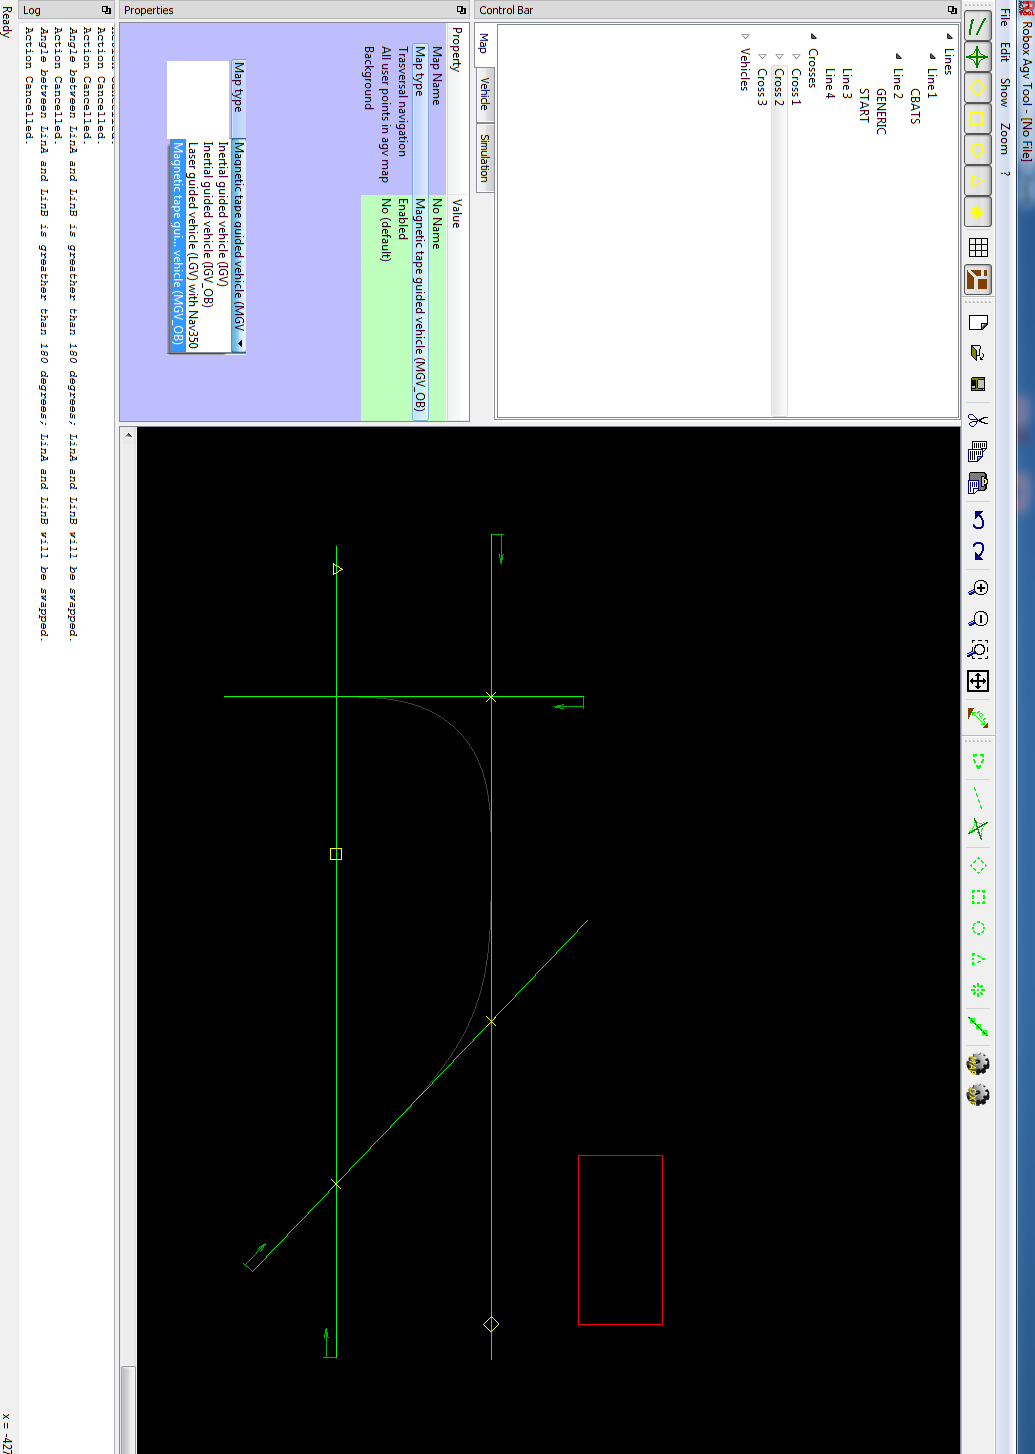
\includegraphics[scale=0.4]{agvmanager/rat/rat}
	\caption{RAT main window}
	\label{fig:refRat}
\end{figure}

\section{Map}
A map is composed by lines, points, crosses and vehicles. During the design of a map some constraint and configuration can be set. For example speed, direction of movement.\\
The main property of a vehicle is the dimension. The length and width can be set here.

\subsection{Vehicle}
We can define the number of vehicles present in a plant, their shapes and dimensions. In our discussion we suppose a vehicle have an orientaion, a coordinate systems attached to it. We can imagine the vectors (arrow) $\overrightarrow{BF}$ and $\overrightarrow{RL}$ as coordinate system axis, fig.\ref{fig:agvOrient}, i.e. $\overrightarrow{x}=\overrightarrow{OF}$ and $\overrightarrow{y}=\overrightarrow{OL}$.\\

If we have more than one Agv, it is convenient to set different colors, we can do it changing the property \textit{Enabled Colour}. The default value is white $(255,255,255)$.

\begin{figure}[h]
	\centering
	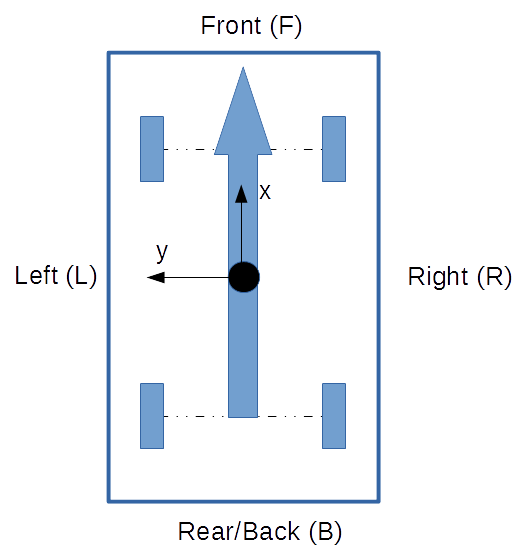
\includegraphics[scale=0.5]{agvmanager/rat/agvOrient}
	\caption{Vehicle orientation}
	\label{fig:agvOrient}
\end{figure}

\subsection{Lines}
A line have mainly 2 properties, beside its location and origin fig.\ref{fig:lineProp}. Navigation direction and vehicle orientation. A line have to be seen as a vector, $\overrightarrow{L}$. For example a vector $\overrightarrow{OX}$ has opposite direction of vector $\overrightarrow{XO}$, note that $\overrightarrow{OX}=-\overrightarrow{XO}$.

Two directions of motion are allowed: Forward and backward. Forward direction is shown by the arrow on the line, that is the positive movement, from $O$ to $X$ represented by $\overrightarrow{OX}$.

The vehicle can move longitudinally fig.\ref{fig:navigLong} to the line, i.e. $\overrightarrow{BF}$ parallel to the line, or transversally (side navigation), i.e. $\overrightarrow{BF}$ perpendicular to the line fig.\ref{fig:navigSide}.

Precisely a line is a vector. The first point drawn $P_{1}$ (first mouse click) define the origin of the vector, the second point $P_{2}$ determine its direction. So the line is defined as $\overrightarrow{P_{1}P_{2}}$. The origin can be moved changing the parameter origin, when it is different from zero we can see the arrow on the line move, the position of the origin is calculated always from $P_{1}$.

\begin{figure}[h]
	\centering
	\begin{subfigure}{0.3\textwidth}
		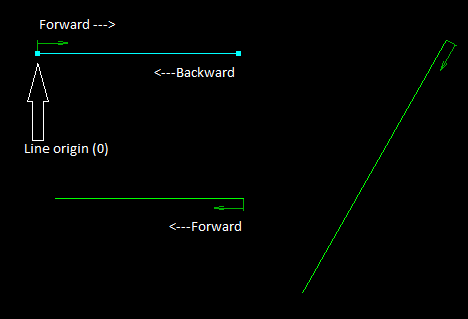
\includegraphics[width=\textwidth]{agvmanager/rat/map_line}
	\caption{Line or vector. Direction of motion}
	\label{fig:mapLine}
	\end{subfigure}
	\quad
	\begin{subfigure}{0.3\textwidth}
		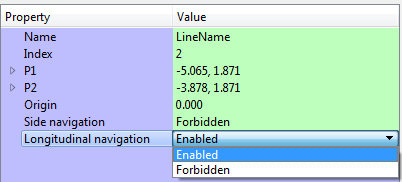
\includegraphics[width=\textwidth]{agvmanager/rat/map_line_prop}
	\caption{Line property. Navigation type can be set : side, longitudinal or both}
	\label{fig:lineProp}
	\end{subfigure}
	\caption{Map line}\label{fig:animals}
\end{figure}


\begin{figure}[h]
	\centering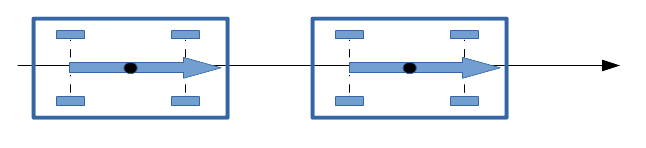
\includegraphics[scale=0.5]{agvmanager/rat/agv_navigation_long}
	\caption{Longitudinal navigation. BF parallel to the line.}
	\label{fig:navigLong}
\end{figure}
\begin{figure}[h]
	\centering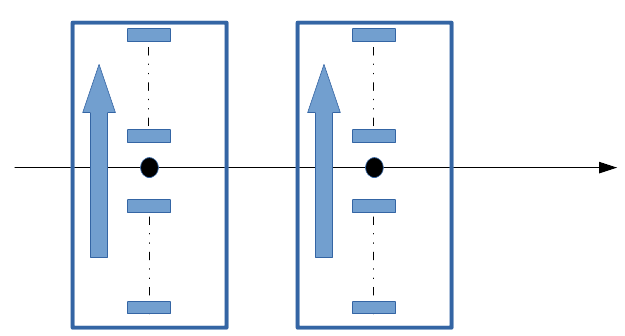
\includegraphics[scale=0.5]{agvmanager/rat/agv_navigation_side}
	\caption{Side or traversal navigation. BF perpendicular to the line.}
	\label{fig:navigSide}
\end{figure}

\subsection{Generic point}
There are 6 kinds of points as shown in fig.\ref{fig:pointKind}. In term of object oriented approach we may say that all points derive from the base class Generic point.
Those points share the following basic properties: Quote (position on the line), speed of the vehicle while crossing the point, direction (as a reference the line where the point is placed) and orientation (referred to the vehicle).

Genric points are used mainly to build the path of the vehicle. It is not necessary to assign a code to a generic point. AgvManager assign codes to Generic points that don't have one.\\

The following discussion can be applied to all kind of points, that have the properties direction and orientation (generic, user, cross, magnet, start, battery).

\begin{figure}[h]
	\centering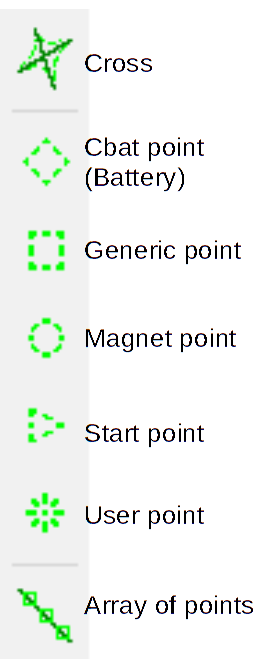
\includegraphics[scale=0.5]{agvmanager/rat/map_points}
	\caption{Kind of points}
	\label{fig:pointKind}
\end{figure}
\begin{figure}[h]
	\centering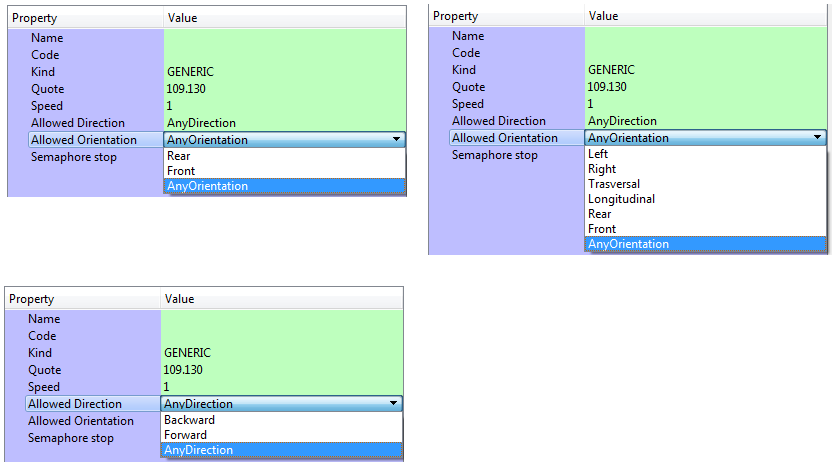
\includegraphics[scale=0.5]{agvmanager/rat/map_point_gen_prop}
	\caption{Generic point property}
	\label{fig:GenericPoint}
\end{figure}

There are three allowed directions to approach and leave a point: Forward(F), Backward (R) and Anydirection (X).
The allowed direction of point e.g.$P_{1}$ is meant as the direction of motion of the vehicle starting from this point toward another point in the positive direction of the line.

For example, if we set the allowed direction of point $P_{1}$ to Forward , and we want to move from $P_{1}$ to point $P_{2}$ placed at a coordinate greater than $P_{1}$, the motion is allowed. But the motion from $P_{2}$ to $P_{1}$ is not allowed. The direction in point $P_{1}$ control the direction of motion starting from itself toward positive coordiantes, fig.\ref{fig:pointdirection}.\\

\begin{figure}[h]
	\centering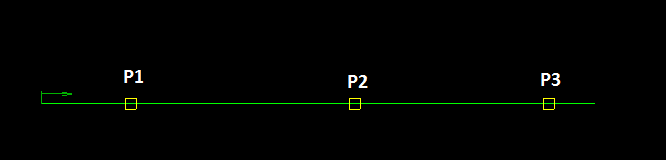
\includegraphics[scale=0.8]{agvmanager/rat/pointdirection}
	\caption{Line from left to right. P1 Forward direction, P2 Backward direction. Motion from P1 to P2 is allowed, from P2 to P1 is not allowed.}
	\label{fig:pointdirection}
\end{figure}
\begin{figure}[h]
	\centering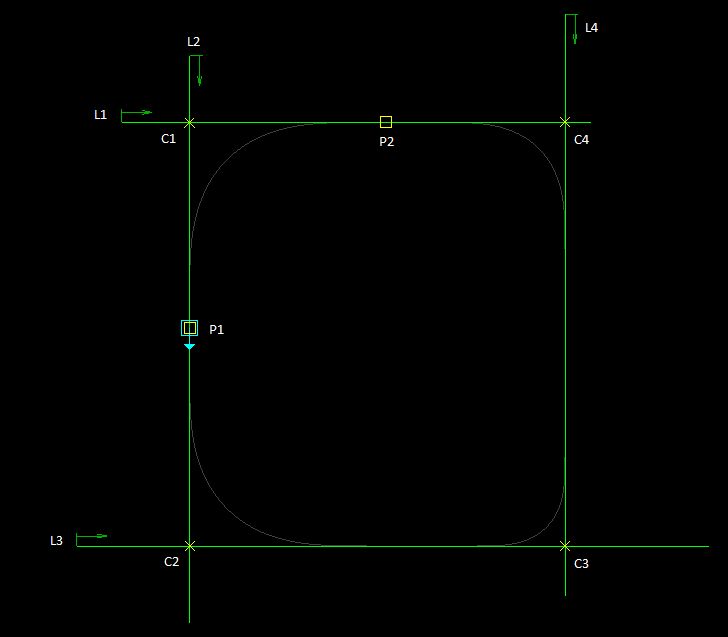
\includegraphics[scale=0.8]{agvmanager/rat/map1}
	\caption{Point allowed direction. $P_{1}$ allowed direction is set to Forward. Motion from $P_{1}$ to $P_{2}$ crossing $C_{1}$ is allowed, because in $C_{1}$ the direction is not restricted, and because $P_{2}$ is not in the growing coordinate starting from $P_{1}$. }
	\label{fig:map1}
\end{figure}

The allowed orientation is referred to the vehicle fig.\ref{fig:agvOrient}. A point have 7 allowed orientations. For example if the Front orientation is selected, the vehicle when is moving on the line, $\overrightarrow{BF}$ have the same orientation of the line $\overrightarrow{L}$. A Front orientation on point $P_{1}$, mean that the vehicle when moving from $P_{1}$ to positive coordinates the orientation of the vehicle is Front.\\

Semaphores can be created using any points except magnet point. When \textit{semaphore index} is 0, there is no semaphore defined. When the index is positive the point define the semaphore start, when it is negative the point define semaphore stop. The semaphore is a rectangluar area, with width define by the parameter \textit{semaphore width}, and length defined by the position of the start and stop points.\\

Speed property????

Can also be created array of points of a selected kind on a line.

\begin{figure}[h]
	\centering
	\begin{subfigure}{0.3\textwidth}
		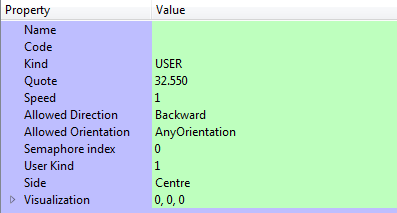
\includegraphics[width=\textwidth]{agvmanager/rat/map_point_user}
		\caption{User point properties}
		\label{fig:userpoint}
	\end{subfigure}
	\begin{subfigure}{0.3\textwidth}
		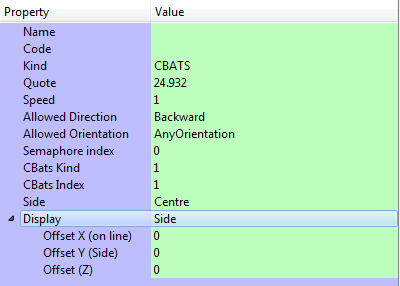
\includegraphics[width=\textwidth]{agvmanager/rat/map_point_cbats}
		\caption{Battery point properties}
		\label{fig:cbatpoint}
	\end{subfigure}
	~ %add desired spacing between images, e. g. ~, \quad, \qquad, \hfill etc. 
	%(or a blank line to force the subfigure onto a new line)
	
	\begin{subfigure}{0.3\textwidth}
		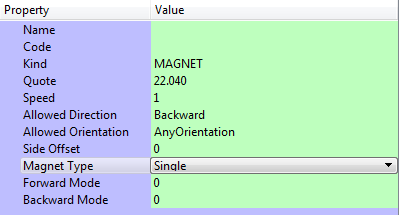
\includegraphics[width=\textwidth]{agvmanager/rat/map_point_magnet}
		\caption{Magnet point properties}
		\label{fig:magnetpoint}
	\end{subfigure}
	~ %add desired spacing between images, e. g. ~, \quad, \qquad, \hfill etc. 
	%(or a blank line to force the subfigure onto a new line)	
	\begin{subfigure}{0.3\textwidth}
		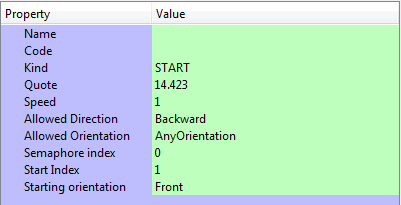
\includegraphics[width=\textwidth]{agvmanager/rat/map_point_start}
		\caption{Start point properties}
		\label{fig:startpoint}
	\end{subfigure}
	
	\caption{Map points}\label{fig:animals}
\end{figure}


\subsection{User point}
User point are like generic point, but they are associated to operations. For example, loading and unloading operations can be associated to user points. Information about the operations done on user points can be written on a database.

A user point should have the code property not empty, but a generic point code could be empty. A point belong to a line, if we have for example a matrix of points and lines, let's suppose the points belong to the horizontal line, if we need to move vertically from a point to another, we can't do it, we need a cross point.


User kind ???????????

Side ?????????????

\subsection{Battery point}
CBats are battery points, i.e. charging station position. This point have the properties kind, index, side and the properties that derive from a generic point fig.\ref{fig:cbatpoint}.

CBats Kind ???????

Side ????????????

Display ?????????????


\subsection{Magnet point}
A magnet point have the similar properties as a generic point, but is not used for path construction. A magnet point is used for position adjustment and reference. Every magnet point should have an Rfid code, this code must be unique.\\

Side offset ???????

Magnet type ???????

Forward mode ?????????/

Backword mode ??????????

A magnet point must be installed at 0.5 m from a curve. For example if we have a cross of type curve, and 1 meter of takeoff distance, 2 magnet points have to be installed at least at 1.5m from the cross \ref{fig:curve_magnet}.

\begin{figure}[h]
	\centering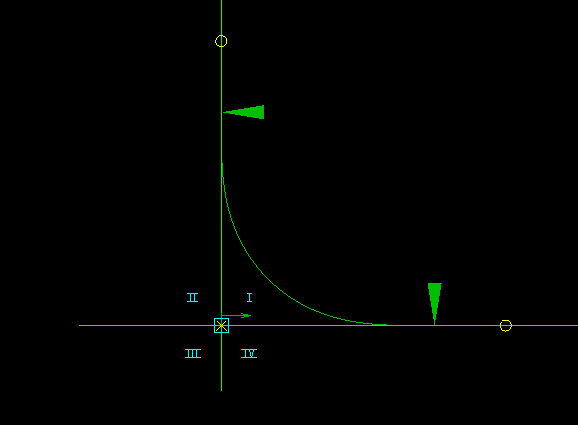
\includegraphics[scale=0.8]{agvmanager/rat/curve_magnet}
	\caption{Two manget points should be place at least 0.5 meter from the end of a curve.}
	\label{fig:curve_magnet}
\end{figure}

%------------------
%
%------------------
\subsection{Start point}
A start point is used as a home reference for a vehicle. A vehicle, once turn on, doesn't know his absolute position. Start point, associated with magnet point can be used to establish the position of a vehicle. In one map we may have more than one start point for one vehicle, pay attention to set the property Start index that should be unique number. If the index is not unique for start points RAT doesn't give any error (like for user points), but AgvManager will give an error when loading the map.\\

A reference position is composed from one start point and 2 magnet points. The position (quote) of the start point should be the same of one of the 2 magnet points.

Starting orientation ??????????

%------------------
%
%------------------
\subsection{Cross}
A cross is the intersection of 2 lines. An intersection have 4 quadrants. You can establish permission for vehicle in one or more quadrants. Three kinds of permission are available: Forbidden, curve and rotation fig.\ref{fig:cross}.

A curve can be of 2 different types: \textcolor{red}{0- Odometric curve} and \textcolor{red}{1- Tape curve with 3 segments}.

\textcolor{blue}{Divieti} is an 8 bit mask, the first 4 bits indicate the allowance of passing from line A to line B, and the second 4 bits indicate teh passing from line B to A.

\textcolor{blue}{Occupable} indicate if the quadrant is occupable, when the agv rotate around itself, if the value is yes, the agv can cross the quadrant while rotating. If all 4 value are no, for the 4 quadrante the agv can only rotate the wheels is the passage mode is rotation.

Under the fields, points on line A and B, we can set the allowed direction an orientations for each line.

Override angle??????/

\begin{figure}[h]
	\centering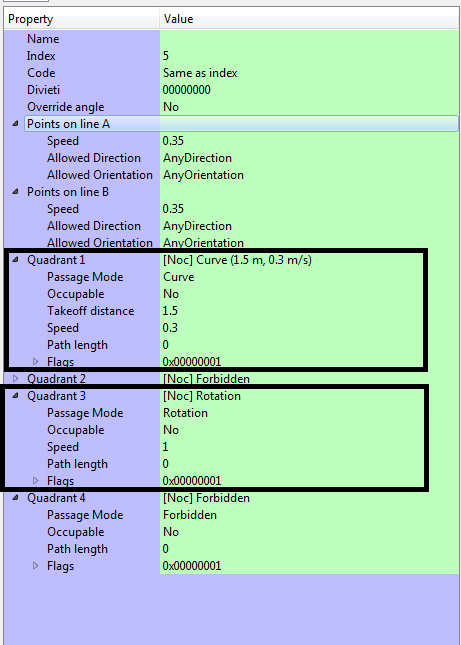
\includegraphics[scale=0.6]{agvmanager/rat/cross}
	\caption{A cross is a point that joint two lines. It behave like a point on every line, orientation and direction can be set for every line independently.}
	\label{fig:cross}
\end{figure}

%------------------
%	Tips
%------------------
\section{Tips}
\begin{enumerate}
	\item A reference point is composed from a start point and 2 magnets.
	\item A curve should have 2 magnets placed at least at 0.5 meter from the end of the curve fig.\ref{fig:curve_magnet}.
	\item User points and generic points should be placed after the magnet points that form the curve fig.\ref{fig:curve_points}.
\end{enumerate}

\begin{figure}[h]
	\centering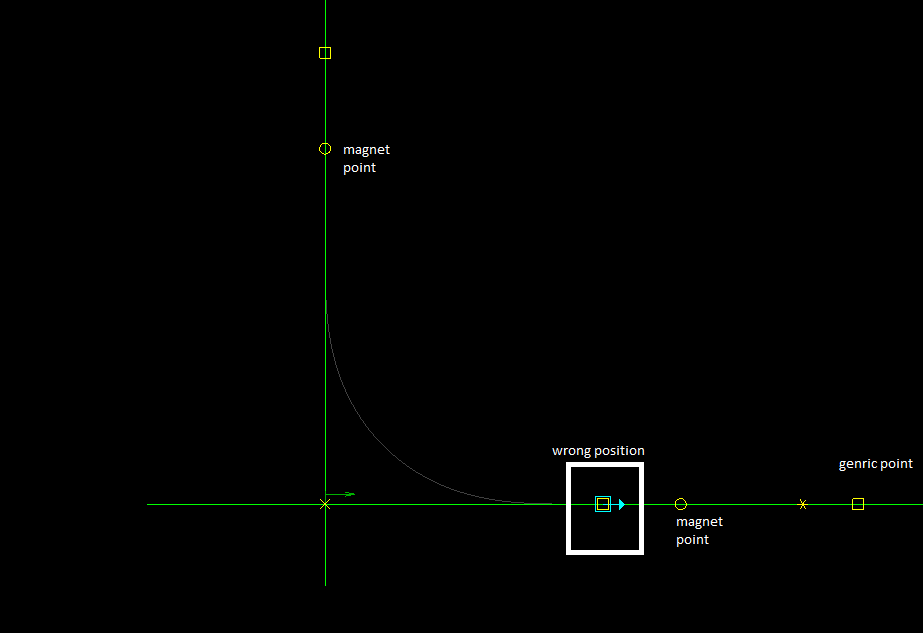
\includegraphics[scale=0.6]{agvmanager/rat/curve_points}
	\caption{Generic points and user points should be placed outside a curve, i.e. after a magnet point.}
	\label{fig:curve_points}
\end{figure}




